\documentclass[journal,12pt,twocolumn]{IEEEtran}
%
\usepackage{setspace}
\usepackage{gensymb}
\usepackage{siunitx}
\usepackage{tkz-euclide} 
\usepackage{textcomp}
\usepackage{standalone}
\usetikzlibrary{calc}
\newcommand\hmmax{0}
\newcommand\bmmax{0}

%\doublespacing
\singlespacing

%\usepackage{graphicx}
%\usepackage{amssymb}
%\usepackage{relsize}
\usepackage[cmex10]{amsmath}
%\usepackage{amsthm}
%\interdisplaylinepenalty=2500
%\savesymbol{iint}
%\usepackage{txfonts}
%\restoresymbol{TXF}{iint}
%\usepackage{wasysym}
\usepackage{amsthm}
%\usepackage{iithtlc}
\usepackage{mathrsfs}
\usepackage{txfonts}
\usepackage{stfloats}
\usepackage{bm}
\usepackage{cite}
\usepackage{cases}
\usepackage{subfig}
%\usepackage{xtab}
\usepackage{longtable}
\usepackage{multirow}
%\usepackage{algorithm}
%\usepackage{algpseudocode}
\usepackage{enumitem}
\usepackage{mathtools}
\usepackage{steinmetz}
\usepackage{tikz}
\usepackage{circuitikz}
\usepackage{verbatim}
\usepackage{tfrupee}
\usepackage[breaklinks=true]{hyperref}
%\usepackage{stmaryrd}
\usepackage{tkz-euclide} % loads  TikZ and tkz-base
%\usetkzobj{all}
\usetikzlibrary{calc,math}
\usepackage{listings}
    \usepackage{color}                                            %%
    \usepackage{array}                                            %%
    \usepackage{longtable}                                        %%
    \usepackage{calc}                                             %%
    \usepackage{multirow}                                         %%
    \usepackage{hhline}                                           %%
    \usepackage{ifthen}                                           %%
  %optionally (for landscape tables embedded in another document): %%
    \usepackage{lscape}     
\usepackage{multicol}
\usepackage{chngcntr}
\usepackage{amsmath}
\usepackage{cleveref}
%\usepackage{enumerate}

%\usepackage{wasysym}
%\newcounter{MYtempeqncnt}
\DeclareMathOperator*{\Res}{Res}
%\renewcommand{\baselinestretch}{2}
\renewcommand\thesection{\arabic{section}}
\renewcommand\thesubsection{\thesection.\arabic{subsection}}
\renewcommand\thesubsubsection{\thesubsection.\arabic{subsubsection}}

\renewcommand\thesectiondis{\arabic{section}}
\renewcommand\thesubsectiondis{\thesectiondis.\arabic{subsection}}
\renewcommand\thesubsubsectiondis{\thesubsectiondis.\arabic{subsubsection}}

% correct bad hyphenation here
\hyphenation{op-tical net-works semi-conduc-tor}
\def\inputGnumericTable{}                                 %%

\lstset{
%language=C,
frame=single, 
breaklines=true,
columns=fullflexible
}
%\lstset{
%language=tex,
%frame=single, 
%breaklines=true
%}
\usepackage{graphicx}
\usepackage{pgfplots}

\begin{document}


\newtheorem{theorem}{Theorem}[section]
\newtheorem{problem}{Problem}
\newtheorem{proposition}{Proposition}[section]
\newtheorem{lemma}{Lemma}[section]
\newtheorem{corollary}[theorem]{Corollary}
\newtheorem{example}{Example}[section]
\newtheorem{definition}[problem]{Definition}
%\newtheorem{thm}{Theorem}[section] 
%\newtheorem{defn}[thm]{Definition}
%\newtheorem{algorithm}{Algorithm}[section]
%\newtheorem{cor}{Corollary}
\newcommand{\BEQA}{\begin{eqnarray}}
\newcommand{\EEQA}{\end{eqnarray}}
\newcommand{\define}{\stackrel{\triangle}{=}}
\bibliographystyle{IEEEtran}
%\bibliographystyle{ieeetr}
\providecommand{\mbf}{\mathbf}
\providecommand{\abs}[1]{\ensuremath{\left\vert#1\right\vert}}
\providecommand{\norm}[1]{\ensuremath{\left\lVert#1\right\rVert}}
\providecommand{\mean}[1]{\ensuremath{E\left[ #1 \right]}}
\providecommand{\pr}[1]{\ensuremath{\Pr\left(#1\right)}}
\providecommand{\qfunc}[1]{\ensuremath{Q\left(#1\right)}}
\providecommand{\sbrak}[1]{\ensuremath{{}\left[#1\right]}}
\providecommand{\lsbrak}[1]{\ensuremath{{}\left[#1\right.}}
\providecommand{\rsbrak}[1]{\ensuremath{{}\left.#1\right]}}
\providecommand{\brak}[1]{\ensuremath{\left(#1\right)}}
\providecommand{\lbrak}[1]{\ensuremath{\left(#1\right.}}
\providecommand{\rbrak}[1]{\ensuremath{\left.#1\right)}}
\providecommand{\cbrak}[1]{\ensuremath{\left\{#1\right\}}}
\providecommand{\lcbrak}[1]{\ensuremath{\left\{#1\right.}}
\providecommand{\rcbrak}[1]{\ensuremath{\left.#1\right\}}}
\theoremstyle{remark}
\newtheorem{rem}{Remark}
\newcommand{\sgn}{\mathop{\mathrm{sgn}}}
\providecommand{\res}[1]{\Res\displaylimits_{#1}} 
%\providecommand{\norm}[1]{\lVert#1\rVert}
\providecommand{\mtx}[1]{\mathbf{#1}}
\providecommand{\fourier}{\overset{\mathcal{F}}{ \rightleftharpoons}}
%\providecommand{\hilbert}{\overset{\mathcal{H}}{ \rightleftharpoons}}
\providecommand{\system}{\overset{\mathcal{H}}{ \longleftrightarrow}}
	%\newcommand{\solution}[2]{\textbf{Solution:}{#1}}
\newcommand{\solution}{\noindent \textbf{Solution: }}
\newcommand{\cosec}{\,\text{cosec}\,}
\providecommand{\dec}[2]{\ensuremath{\overset{#1}{\underset{#2}{\gtrless}}}}
\newcommand{\myvec}[1]{\ensuremath{\begin{pmatrix}#1\end{pmatrix}}}
\newcommand{\mydet}[1]{\ensuremath{\begin{vmatrix}#1\end{vmatrix}}}
%\numberwithin{equation}{section}
\numberwithin{equation}{subsection}
%\numberwithin{problem}{section}
%\numberwithin{definition}{section}
\makeatletter
\@addtoreset{figure}{problem}
\makeatother
\let\StandardTheFigure\thefigure
\let\vec\mathbf
%\renewcommand{\thefigure}{\theproblem.\arabic{figure}}
\renewcommand{\thefigure}{\theproblem}
%\setlist[enumerate,1]{before=\renewcommand\theequation{\theenumi.\arabic{equation}}
%\counterwithin{equation}{enumi}
%\renewcommand{\theequation}{\arabic{subsection}.\arabic{equation}}
\def\putbox#1#2#3{\makebox[0in][l]{\makebox[#1][l]{}\raisebox{\baselineskip}[0in][0in]{\raisebox{#2}[0in][0in]{#3}}}}
     \def\rightbox#1{\makebox[0in][r]{#1}}
     \def\centbox#1{\makebox[0in]{#1}}
     \def\topbox#1{\raisebox{-\baselineskip}[0in][0in]{#1}}}
\vspace{3cm}
\title{Assignment-6\\}
\author{Hrithik Raj}
\maketitle
\newpage
%\tableofcontents
\bigskip
\renewcommand{\thefigure}{\theenumi}
\renewcommand{\thetable}{\theenumi}
\begin{abstract}
This document contains solution of Problem Ramsey\brak{4.1.4}
\end{abstract}
Download latex-tikz codes from 
%
\begin{lstlisting}
https://github.com/Hrithikraj2/MatrixTheory_EE5609/blob/master/Assignment_6/A6.tex
\end{lstlisting}
\section{\textbf{Question}}
Trace the parabola
\begin{align}\nonumber
    16x^2+24xy+9y^2-5x-10y+1 = 0
\end{align}
\section{Solution}
Compare the given equation with the standard form
\begin{align}\label{eq:1}
    ax^2+2bxy+cy^2+2dx+2ey+f = 0
\end{align}
Write the values Of V and u as follows
\begin{align}
    \vec{V} = \vec{V}^T = \myvec{16 & 12\\12 & 9} \quad
    \vec{u} =\myvec{-\frac{5}{2} \\ -5} \quad
     f = 1 \label{eq:2}
\end{align}
The characteristic equation of $\vec{V}$ is given as
\begin{align}
    \mydet{\lambda\vec{I}-\vec{V}} = 0\\
    \implies \mydet{\lambda-16 & -12 \\ -12 & \lambda-9} = 0\\
    \implies \lambda^2 -25\lambda = 0 \label{eq:3}
\end{align}
The eigenvalues are the roots of the equation \eqref{eq:3} are
\begin{align}
    \lambda_{1} = 0, \quad \lambda_{2} = 25 \label{eq:4}
\end{align}
The eigen vector $\vec{p}$ is defined as, 
\begin{align}
    \vec{V}\vec{p} &= \lambda\vec{p}\\
    \implies(\lambda\vec{I}-\vec{V})\vec{p}&=0
\end{align}
For $\lambda_1=0$
\begin{align}
    (\lambda_1\vec{I}-\vec{V}) = \myvec{-16 & -12\\-12 & -9}\xleftrightarrow[R_2\leftarrow R_2-3R_1]{R_1\leftarrow \frac{1}{4}R_1}\myvec{-4 & -3\\0 & 0}
\end{align}
\begin{align}
    \implies\vec{p_1}&=\frac{1}{5}\myvec{-3\\4}\label{eq:p1val}
\end{align}
For $\lambda_2=25$
\begin{align}
    (\lambda_2\vec{I}-\vec{V}) = \myvec{9 & -12\\-12 & 16}\xleftrightarrow[R_2\leftarrow R_2+4R_1]{R_1\leftarrow \frac{1}{3}R_1}\myvec{3 & -4\\0 & 0}
\end{align}
\begin{align}
    \implies\vec{p_2}=\frac{1}{5}\myvec{4\\3}\label{eq:p2val}
\end{align}
Use Eigenvalue decomposition, $\vec{P}^T\vec{V}\vec{P}=\vec{D}$, where
\begin{align}
    \vec{P} = \frac{1}{5}\myvec{-3 & 4\\4 & 3}\\
    \vec{D} = \myvec{\lambda_1 & 0\\0 & \lambda_2} = \myvec{0 & 0\\ 0 & 25}
\end{align}
Focal length of the parabola is given as
\begin{align}
    \text{focal length} = \abs{\frac{2\eta}{\lambda_2}}\label{eq:fl}\\
    \eta = \vec{p}_1^T\vec{u} = -\frac{5}{2}\label{eq:eta}\\
    \intertext{Substituting values from \eqref{eq:eta} and \eqref{eq:4} in \eqref{eq:fl}, we get}
    \text{focal length} = \frac{1}{5}
\end{align}
The standard equation of the parabola is given by
\begin{align}
    \vec{y}^T\vec{D}\vec{y} = -2\eta\myvec{1 & 0}\vec{y}
\end{align}
And the vertex $\vec{c}$ is given by
\begin{align}
    \myvec{\vec{u}^T + \eta\vec{p}_1^T \\ \vec{V}}\vec{c} = \myvec{-f \\ \eta\vec{p}_1 - \vec{u}} \label{eq:c}
\end{align}
Substituting values from \eqref{eq:2},\eqref{eq:eta},\eqref{eq:p1val} in \eqref{eq:c},
\begin{align}
    \myvec{-4 & -7\\16 & 12\\12 & 9}\vec{c} = \myvec{-1\\4\\3}
\end{align}
To find $\vec{c}$, performing row reduction on the augmented matrix as follows:
\begin{align}
    \myvec{-4 & -7 & -1\\16 & 12 & 4\\12 & 9 & 3}\xleftrightarrow[R_1\leftarrow \frac{-1}{4}R_1]{R_3\leftarrow R_3-\frac{3}{4}R_2}\myvec{1 & \frac{7}{4} & \frac{1}{4}\\16 & 12 & 4\\0&0&0}\\
    \xleftrightarrow{R_2\leftarrow R_2-16R_1}\myvec{1 & \frac{7}{4} & \frac{1}{4}\\0 & -16 & 0\\0&0&0}\\\xleftrightarrow{R_2\leftarrow \frac{-1}{16}R_2}\myvec{1 & \frac{7}{4} & \frac{1}{4}\\0 & 1 & 0\\0&0&0}\\\xleftrightarrow{R_1\leftarrow R_1-\frac{7}{4}R_2}\myvec{1 & 0 & \frac{1}{4}\\0 & 1 & 0\\0&0&0}
\end{align}
Thus,
\begin{align}
    \vec{c} = \myvec{\frac{1}{4}\\0} %= \myvec{-2.4 \\ -1.8}
\end{align}
\renewcommand{\thefigure}{1}
\begin{figure}[h!]
    \centering
    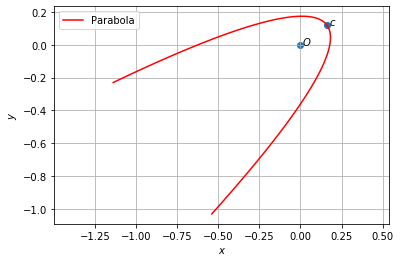
\includegraphics[width=\columnwidth]{A6.png}
    \caption{Parabola with vertex c}
    \label{fig:fig1}
\end{figure}
\end{document}